\chapter[Appendix]{}
\label{chap:appendix}

A few experiments / results that are not that relevant for the scope of this thesis are mentioned in this chapter.

\section{Sampler parallelization}
\label{sec:sampler_parallelization}
Figure \ref{fig:sampler_parallelization} shows the benchmark results between the naive sampler with and without parallelization.
The benchmark was performed on a singular NVIDIA Ampere A100 GPU.
\begin{figure}[h]
    \centering
    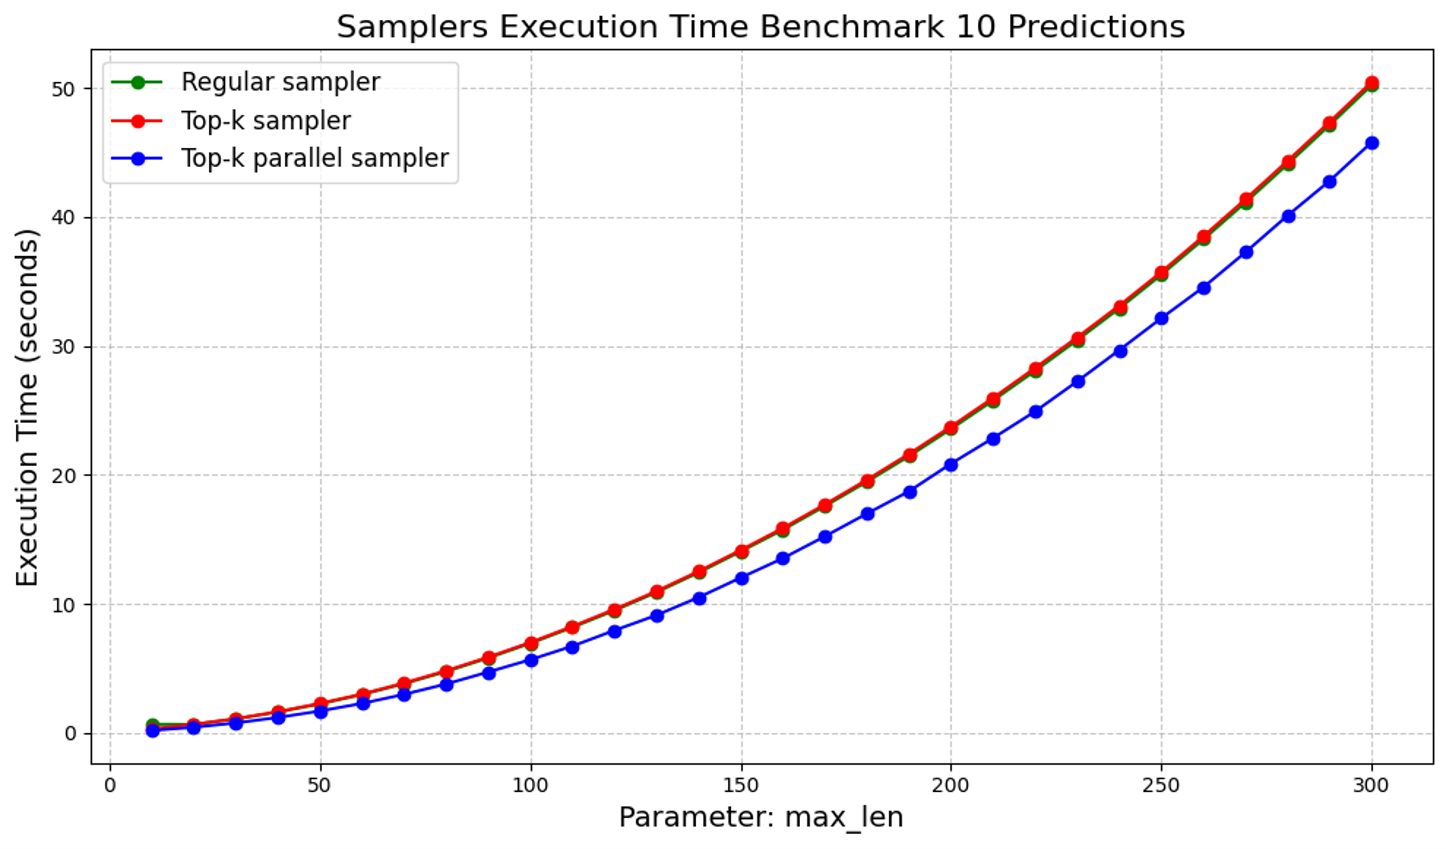
\includegraphics[width=0.6\linewidth]{figures/appendix/sampler_parallel.png}
    \caption{Execution Time Benchmark sampler parallelization}
    \label{fig:sampler_parallelization}
\end{figure}

The naive sampler shows to be more computationally efficient with parallelization.
A small difference in execution time can be substantial when this sampler is called thousands of times.
All further stochastic samplers in this thesis were executed with this parallelization enabled.

\section{Stochastic samplers benchmark full results}
\label{sec:sampler_full_results}

Figures \ref{fig:top-k_appendix}, \ref{fig:top-k_zoomed_appendix}, \ref{fig:top-p_appendix}, \ref{fig:top-p_zoomed_appendix} show the full results from the top-k and top-p benchmark.

\begin{figure}[h]
    \centering
    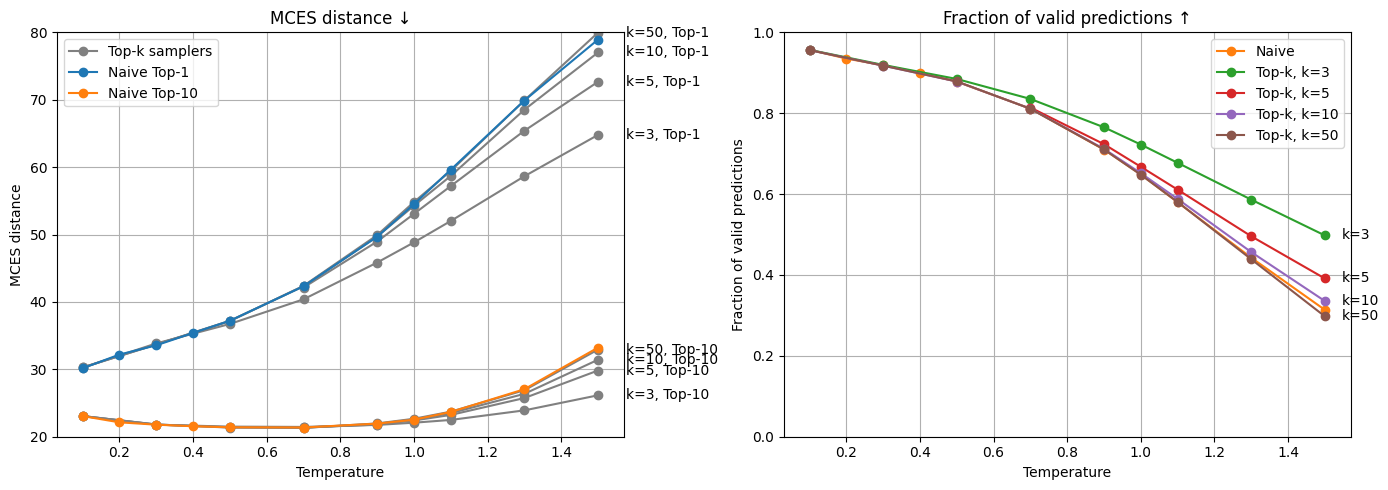
\includegraphics[width=\linewidth]{figures/appendix/samplers/top-k_vs_naive.png}
    \caption{Full top-k benchmark with top-1 and temperature search results on the validation set}
    \label{fig:top-k_appendix}
\end{figure}

Top-k with $k=20$ is left out of figure \ref{fig:top-k_appendix} for readability. These results are in line with the others.

\begin{figure}[h]
    \centering
    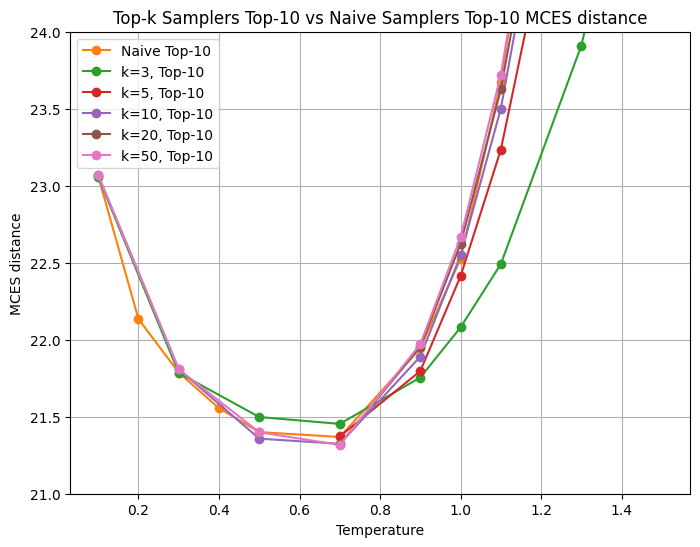
\includegraphics[width=0.6\linewidth]{figures/appendix/samplers/top-k_vs_naive_top-10.png}
    \caption{Zoomed in top-k top-10 MCES distance on the validation set}
    \label{fig:top-k_zoomed_appendix}
\end{figure}

Figure \ref{fig:top-k_zoomed_appendix} shows the slight improvement of top-k $k\geq 10$ to the naive sampler in the temperature optima.

\begin{figure}[h]
    \centering
    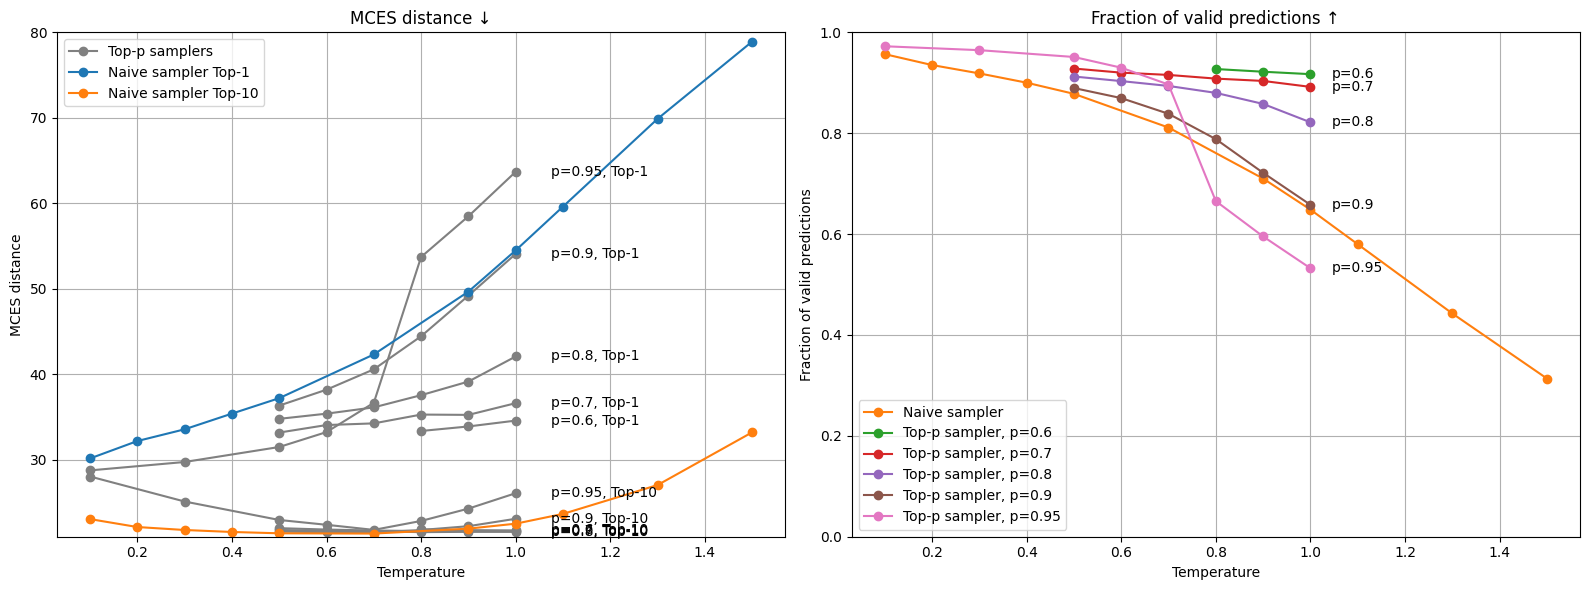
\includegraphics[width=\linewidth]{figures/appendix/samplers/top-p_vs_naive.png}
    \caption{Full top-p benchmark with top-1 and temperature search results on the validation set}
    \label{fig:top-p_appendix}
\end{figure}

The search grid for the top-p benchmark was for some values of $p$ cut short to save resources.

\begin{figure}[h]
    \centering
    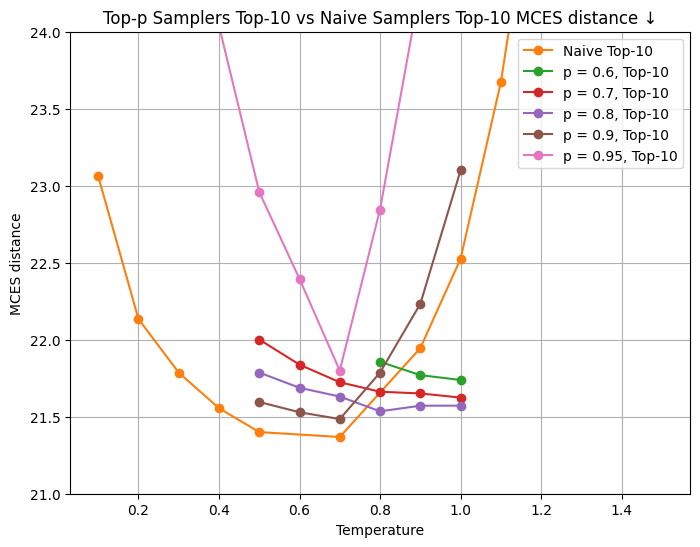
\includegraphics[width=0.6\linewidth]{figures/appendix/samplers/top-p_vs_naive_top-10.png}
    \caption{Zoomed in top-p top-10 MCES distance on the validation set}
    \label{fig:top-p_zoomed_appendix}
\end{figure}

Figure \ref{fig:top-p_zoomed_appendix} shows that the top-p sampler results do not exceed the results from the naive sampler in their temperature optima.


\section{Top-10 Naive sampler temperature search results}
This section shows the full naive top-10 results of the \ac{BPE}, augmentation and molecular representations experiments for different temperatures.
\label{sec:temp_search_appendix}

\subsection*{BPE as pretraining}
\begin{figure}[h!]
    \centering
    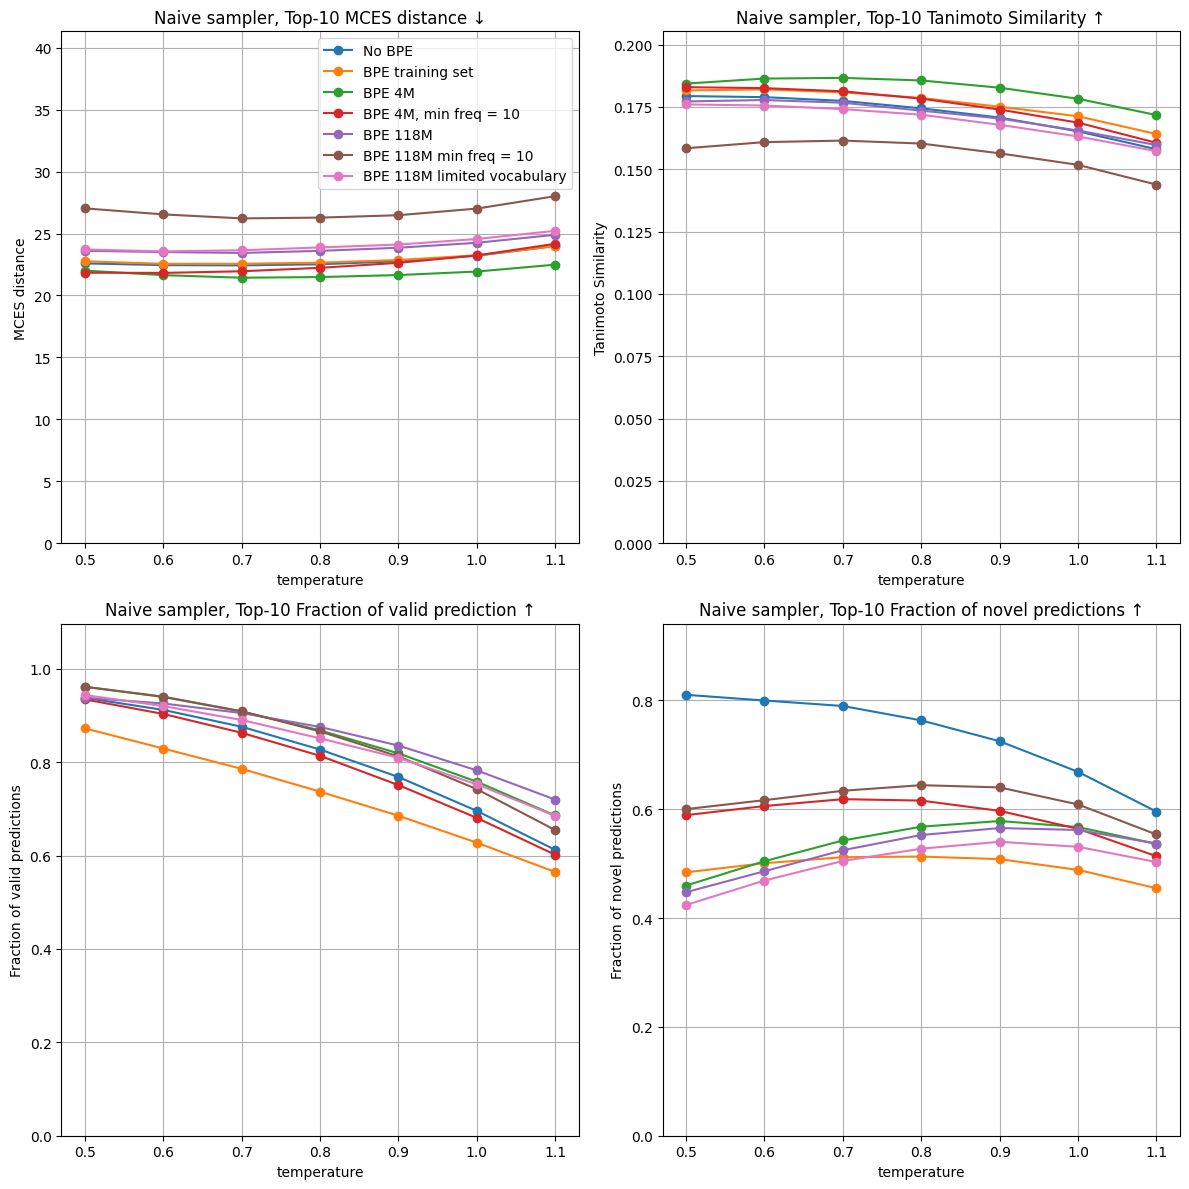
\includegraphics[width=1.0\textwidth]{figures/appendix/bpe_with_tanimoto.png}
    \caption{Top-10 Naive sampler temperature search BPE experiment results on the validation set}
    \label{fig:bpe_appendix}
\end{figure}

\subsection*{Augmentation}
\begin{figure}[H]
    \centering
    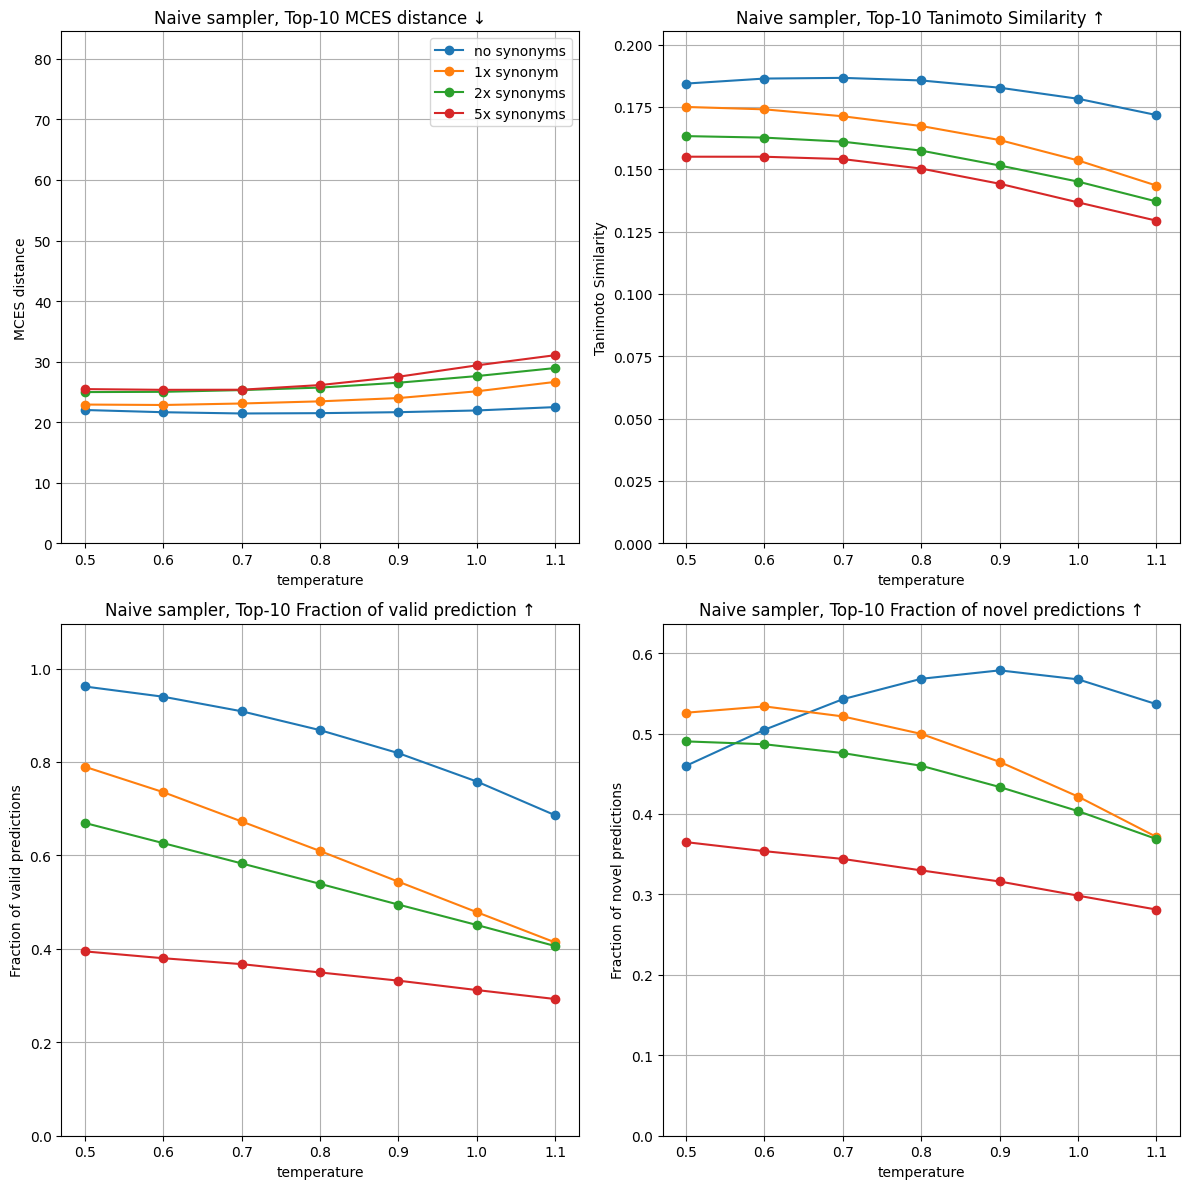
\includegraphics[width=1.0\textwidth]{figures/appendix/smiles_augmentation_with_tanimoto.png}
    \caption{Top-10 Naive sampler temperature search smiles augmentation experiment results on the validation set}
    \label{fig:smiles_augmentation_appendix}
\end{figure}

\begin{figure}[H]
    \centering
    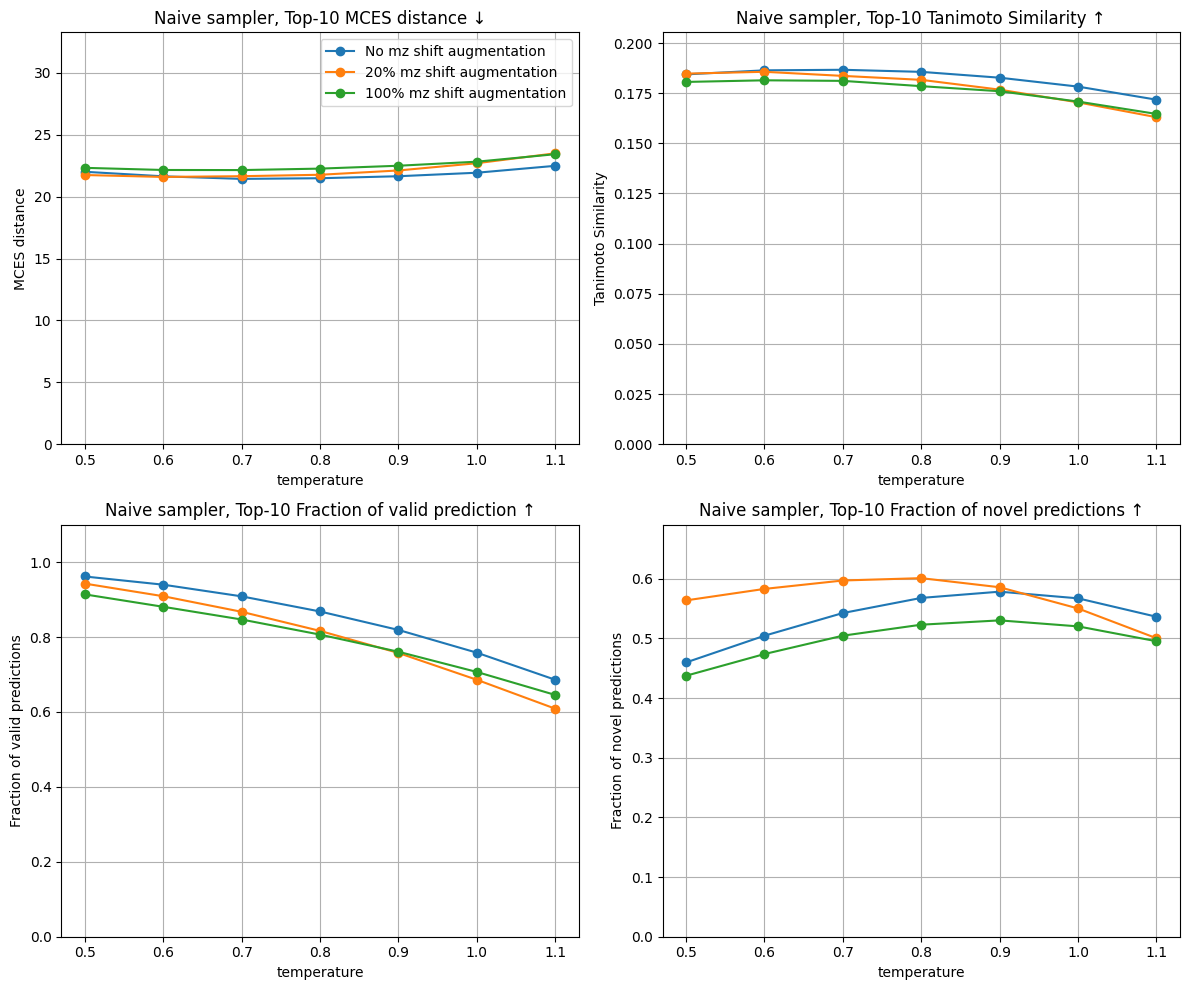
\includegraphics[width=1.0\textwidth]{figures/appendix/spectal_augmentation_with_tanimoto.png}
    \caption{Top-10 Naive sampler temperature search spectral augmentation experiment results on the validation set}
    \label{fig:spectral_augmentation_appendix}
\end{figure}

\subsection*{Representations}
\begin{figure}[H]
    \centering
    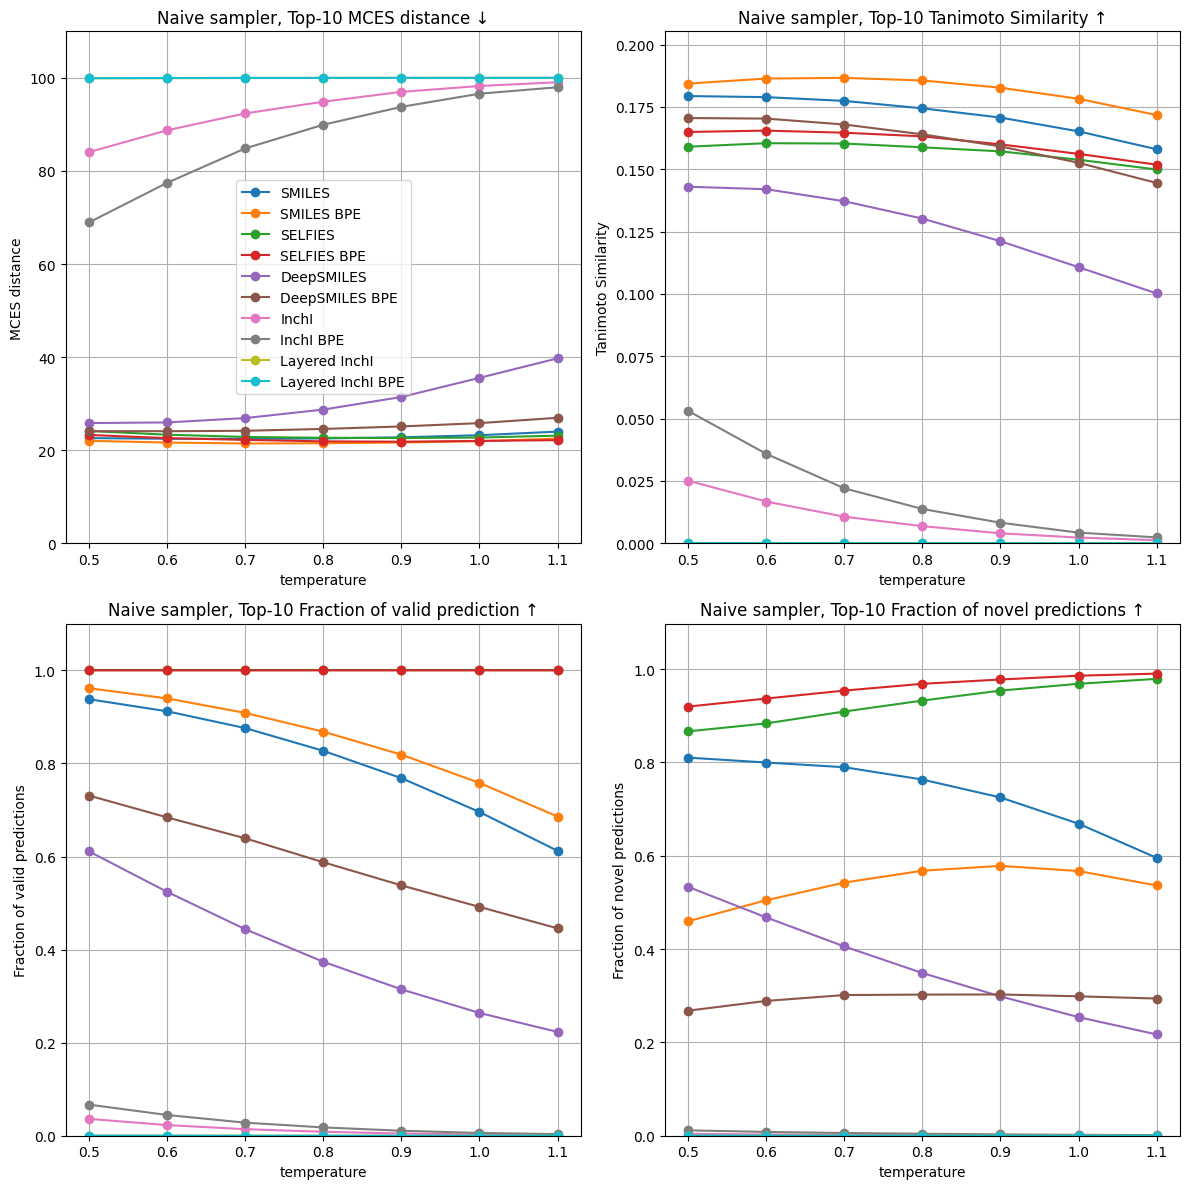
\includegraphics[width=1.0\textwidth]{figures/appendix/representations_with_layered_inchi_with_tanimoto.png}
    \caption{Top-10 Naive sampler temperature search representations experiment results on the validation set}
    \label{fig:representations_appendix}
\end{figure}

\begin{figure}[H]
    \centering
    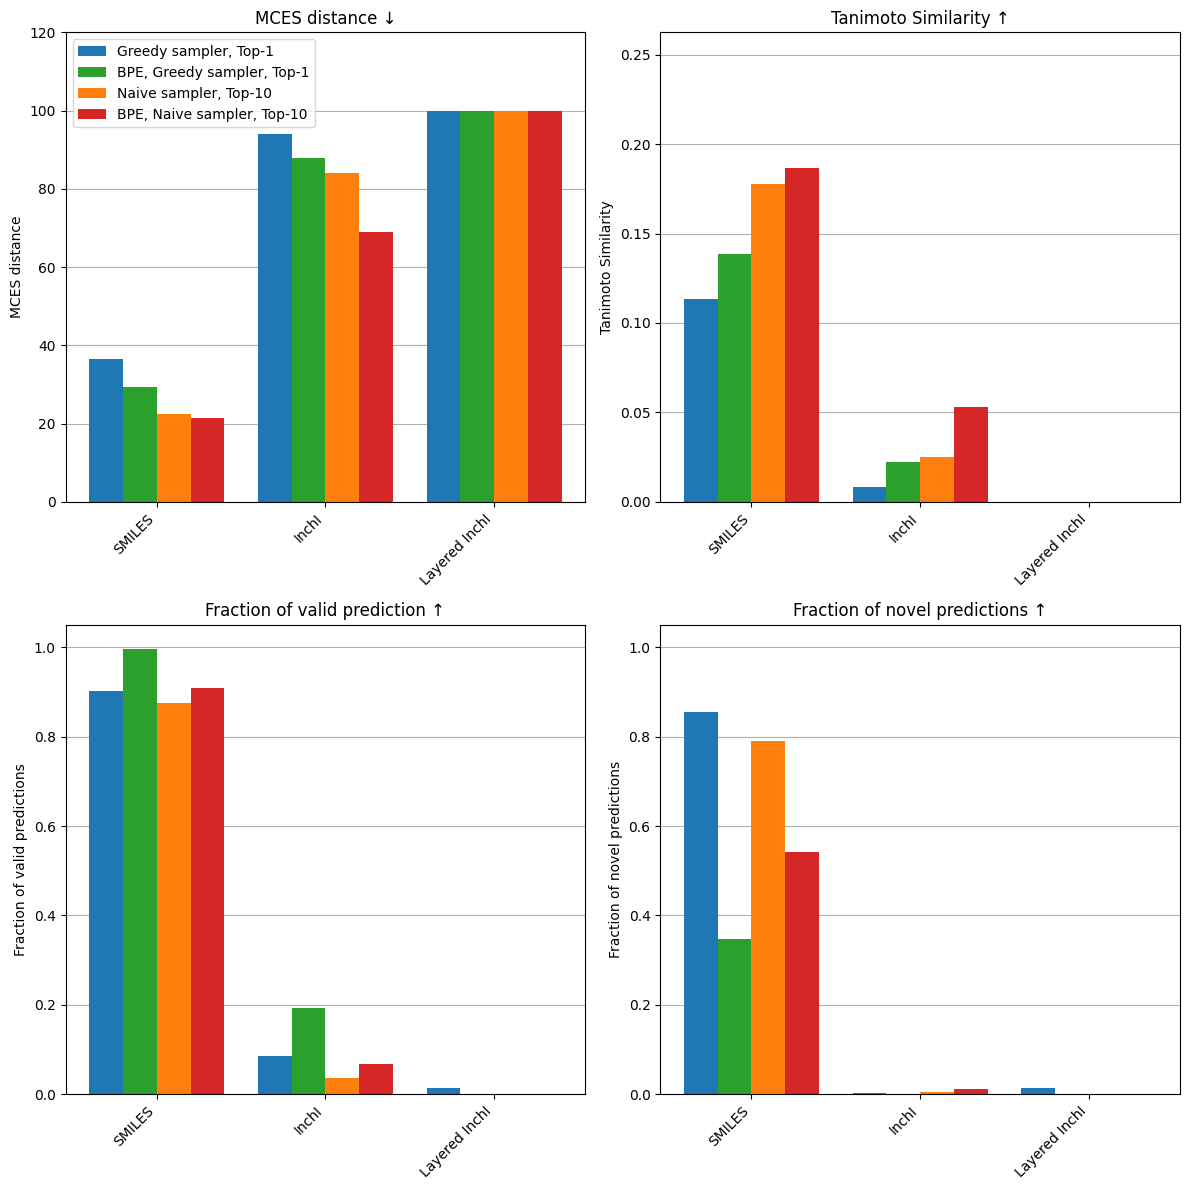
\includegraphics[width=1.0\textwidth]{figures/appendix/layered_inchi_with_tanimoto.png}
    \caption{Evaluation on the validation set of three-headed InchI model compared to the SMILES and InchI models}
    \label{fig:layered_inchi}
\end{figure}

Figure \ref{fig:layered_inchi} shows the performance of the InchI model with three decoders. It is clear the the model struggles to predict any valid molecules.